% THIS IS SIGPROC-SP.TEX - VERSION 3.1
% WORKS WITH V3.2SP OF ACM_PROC_ARTICLE-SP.CLS
% APRIL 2009
%
% It is an example file showing how to use the 'acm_proc_article-sp.cls' V3.2SP
% LaTeX2e document class file for Conference Proceedings submissions.
% ----------------------------------------------------------------------------------------------------------------
% This .tex file (and associated .cls V3.2SP) *DOES NOT* produce:
%       1) The Permission Statement
%       2) The Conference (location) Info information
%       3) The Copyright Line with ACM data
%       4) Page numbering
% ---------------------------------------------------------------------------------------------------------------
% It is an example which *does* use the .bib file (from which the .bbl file
% is produced).
% REMEMBER HOWEVER: After having produced the .bbl file,
% and prior to final submission,
% you need to 'insert'  your .bbl file into your source .tex file so as to provide
% ONE 'self-contained' source file.
%
% Questions regarding SIGS should be sent to
% Adrienne Griscti ---> griscti@acm.org
%
% Questions/suggestions regarding the guidelines, .tex and .cls files, etc. to
% Gerald Murray ---> murray@hq.acm.org
%
% For tracking purposes - this is V3.1SP - APRIL 2009

\documentclass{acm_proc_article-sp}

% gets rid of copyright block 
\makeatletter
\def\@copyrightspace{\relax}
\makeatother

\begin{document}

\title{A Web Interface Usability Evaluation of a Public Collaborative Data Portal}
% \subtitle{[Extended Abstract]}

\numberofauthors{4} 
\author{
% \alignauthor
% Author One\titlenote{Now on postdoctoral fellow at ABC University}\\
%       \affaddr{Institute One}\\
%       \affaddr{Address One}\\
%       \email{author.one@emails.com}
\alignauthor
Vinh Le\\
       \affaddr{University of Nevada, Reno}\\
       \affaddr{1664 N. Virginia St.}\\
       \affaddr{Reno, NV 89557}\\
       \email{vdacle@gmail.com}
% \and % go to new row
\alignauthor
Terence Henriod \\
       \affaddr{University of Nevada, Reno}\\
       \affaddr{1664 N. Virginia St.}\\
       \affaddr{Reno, NV 89557}\\
       \email{thenriod@gmail.com}
\alignauthor
Sergiu Dascalu\\
       \affaddr{University of Nevada, Reno}\\
       \affaddr{1664 N. Virginia St.}\\
       \affaddr{Reno, NV 89557}\\
       \email{dascalus@cse.unr.edu}
}

\date{\today}


\maketitle
\begin{abstract}
The Nevada Research Data Center(NRDC) is a data portal sponsored by The National Science Foundation and hosts a number of data services that affords users access to climate data from project sites throughout Nevada. This paper entails a study of the usability of these data services and layout across two versions of the NRDC portal, the current production version and a new in-development version. The experiment features a series of tasks in which subjects of the study undertake for each iteration and service, and providing feedback. Overall, participants of this study required 90 to 100 seconds and 30 to 100 mouse clicks to complete tasks, while following usage averaged 30 seconds and 15 mouse clicks. This implied a strong learning curve on each of the data services with the open chance of a user being overtly lost. Additionally, feedback from participants indicated an average preference rating of 4.0 where 1 represents a strong preference for the current iteration of the NRDC interface and 5 being the in-development iteration. From these results, participants have shown a full preference to the in-development iteration. 
\end{abstract}

% A category with the (minimum) three required fields
% \category{H.4}{Information Systems Applications}{Miscellaneous}
\category{H.5.2}{User Interfaces}{Screen design (e.g., text, graphics, color), Graphical user interfaces (GUI), Ergonomics, Evaluation/methodology.}
%A category including the fourth, optional field follows...
% \category{D.2.8}{Software Engineering}{Metrics}[complexity measures, performance measures]

\terms{Human Factors, Human-Computer Interaction (HCI), Design, Performance}

\keywords{Aesthetics, Attractiveness, Web Design, Search Perseverance} % NOT required for Proceedings

%
%
\section{Introduction}
%
\subsection{NRDC}
The Nevada Research Data Center, formerly the Nevada Climate Change Portal (NCCP),  is a web portal that grants specific climate data services to researchers. The NRDC and NCCP were born of The Solar Energy Water Environment Nexus Project, a National Science Foundation funded venture into establishing Nevada as a competitive state for climate research \cite{nvsolarnexus.org}. The purpose of the NRDC is to serve as a aggregation hub to gather and distribute climate data streaming from research sites created across Nevada. The NRDC mission statement is "To facilitate the storage, retrieval, and analysis of research data that is relevant to the needs and interests of the state of Nevada." \cite{nccp,nrdc} 

Use of the NRDC has grown exponentially over the past two years; its initial user base started with a select few individuals and has grown to nearly three thousand users. New services are added routinely as the system encompasses more projects. As development continues for the NRDC, it is vital that the current services are continually optimized for a better user end experience or else risk a loss of attraction in the eyes of its users\cite{usability.gov}. The idea of this project is to perform a user study on the main services present within the system in order to extrapolate a plausible future direction for the NRDC. In this user study, participants will be utilizing the already developed web services located on the NRDC, whilst providing feedback based on ease of usage.

One of the main ideals that make up Human and Computer Interaction (HCI) is the pursuit or development of a better user end experience\cite{hci-research-perspective}. As this study is designed to find a form of better usability on a web interface, this project holds a great deal of relevancy to the field of HCI \cite{web-ui-principles,dontmakemethink}. The NRDC is heavily affiliated with the Department of Computer Science and Engineering (CSE), which allows for an easier access to references and support, thus making the choice of having this user study very attractive. Additionally, this study would benefit the members of the CSE department, as well as the National Science Foundation, making this a fantastic choice to give back to the both organizations, as we have been affiliated with them in the past.

%
\subsection{Related Work}
This paper is not the first time an effort was made to improve the already existing NRDC system. Microservice-based Architecture for the NRDC was a recent improvement brought around to update the system into a more scalable and stable architecture. The microservices in question would allow the system to retain service if one of the databases were to suddenly fail. This would enable the portal to remain online and provide any services still active, instead of bringing down the entire system all at once \cite{microservice-nrdc}.

Additionally, this is not the first time a web interface was tested for usability. The works of I. Nakarada-Kordic and B. Lobb guided the design of this experimental study. Their work detailed research on web interface usability by employing visual search tasks on various websites. The clever use of using metrics such as accuracy, task time, and perseverance inspired the path in which we chose. Nakarada-Kordic and Lobb eventually came to the conclusion that the perceived attractiveness of the interface directly affected the search perseverance \cite{PerceivedAttractiveness}. 

In the following sections, we describe our experimental method. This will compose of our criteria of participants, our choice of apparatus, the actual process of our experiment, and the final design of the study. Following this, we present our results along with plans for future development.

%
%
\section{Method}
%
\subsection{Participants}
Eight (8) participants were gathered. Participants included undergraduate and graduate students and faculty of the University of Nevada, Reno. Students and faculty were chosen primarily because they are representative of the researcher population.

Participants were solicited in person and chosen on the basis of having no exposure to the NRDC (most participants had no awareness of the NRDC at all; uninitiated users are considered good candidates for revealing usability flaws\cite{dontmakemethink}). Participants were compensated with refreshments (chips and a drink) for their participation. There was no formal selection process, selection of participants was random.

%
\subsection{Apparatus}
The experiment was conducted in a quiet, graduate student group workspace in the Cyber-Infrastructure Lab (CI Lab) of UNR. The experiment was carried out using a standard desktop computer work station, a simple phone application for giving tasks to participants, and the researchers themselves. The tasks themselves and the data collected are also described in this section.

Participants were asked to access and use the NRDC web portal using a work station with a standard keyboard and mouse. The computer had a common web browser (Google Chrome) open and full-screened, so participants' attention would be fully focused on the use of the NRDC. The web browser featured only three (3) bookmarks for easy navigation: "NRDC A", "NRDC 1", and "Q" (aliases for the \emph{current} and \emph{in-development} versions of the NRDC and the post experiment survey, respectively). The bookmarks were named to minimize distraction and mask the identities of the NRDC interfaces without introducing bias.

\begin{figure}[h!]
  \centering
  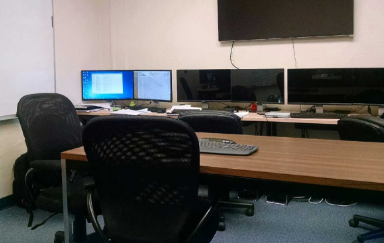
\includegraphics[width=.8\linewidth]{ci_lab_apparatus}
  \caption{The experiment location: The Cyber-Infrastructure Lab of UNR.}
  \label{fig:ci_lab}
\end{figure}

The phone application was a custom-made Android application named "HCI-Task". The purpose of this application was to have a medium separate from the workstation to deliver the tasks participants would be asked to complete, so as not to take screen space from the NRDC. HCI-Task presented textual descriptions of tasks and screen-shots indicating the final, correct result of the task. HCI-Task collected timings for task completions, and presented buttons for the participant to indicate if they completed the task or if they chose to give-up on the task.

\begin{figure}[h!]
  \centering
  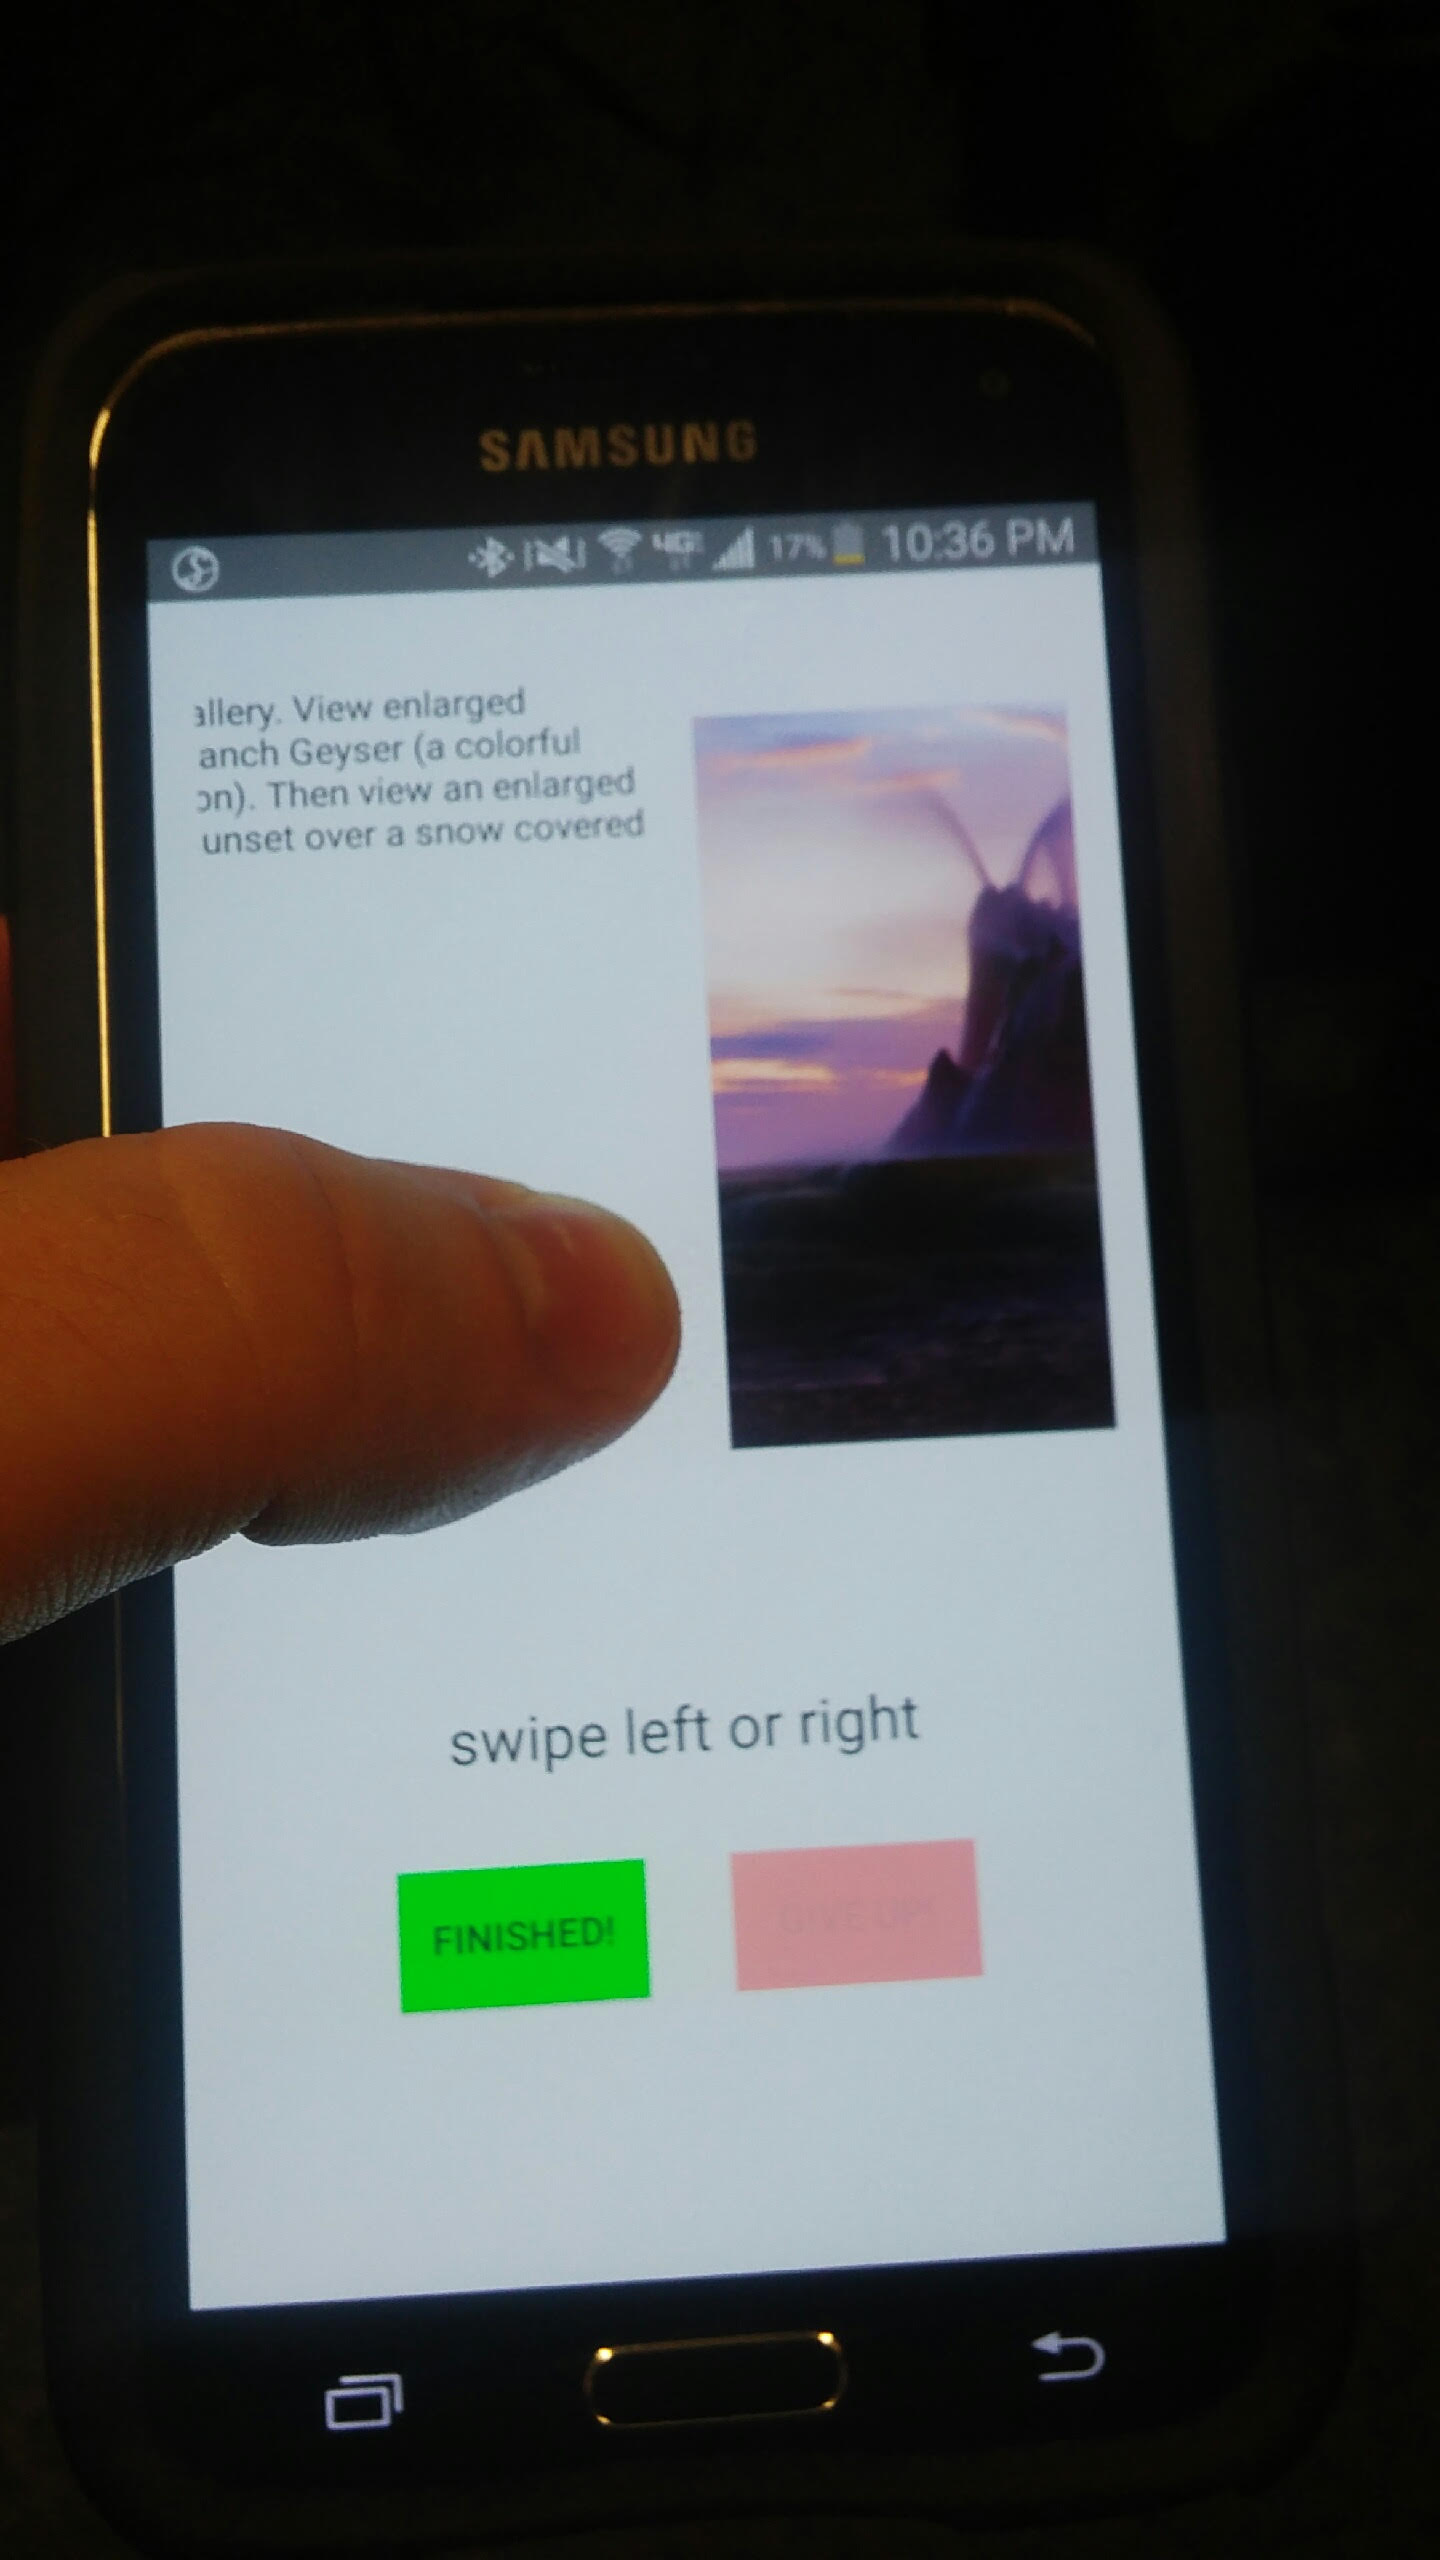
\includegraphics[width=.3\linewidth]{task_app}
  \caption{The task-dispensing app used to give participants tasks. In this image, the user is alternating between a text description of the task and a screen-shot of the desired result.}
  \label{fig:task_app}
\end{figure}

Given the difficulty of instrumenting the NRDC and the computer used by participants, some data was collected manually by the researchers. The researchers counted clicks on each task, observed certain behaviors and events, and verified if a participant had correctly completed a task.

%
\subsection{Procedure}
The experiment procedure lasted from 30 minutes to an hour. After being contacted and brought to the CI Lab, participants were seated at the experiment work station. Participants were then greeted and read a short script indicating their rights and the nature of the experiment they were about to participate in.

Two task sets were formulated for participants. Each task set contained seven (7) tasks, which consisted of: one (1) use of the Current Conditions service, two (2) Geo-spatial Data Search tasks, two (2) WebCam Image Archive service tasks, one (1) Image Archive or About Us task, and finally one (1) task to retrieve information on an NRDC connection (or partner). The tasks all varied in the type of information to be gathered, and the order of tasks was the same in both sets to help control for order-effects. 

The experiment was carried out in the following steps, with scripted instructions read at each step:
\begin{enumerate}
\item \textbf{Briefing}
Participants were briefed on the purpose of the NRDC and the nature of the experiment. They were introduced to the parts of the experiment apparatus, but not what data was being collected to prevent participants from behaving unnaturally.

\item \textbf{Training}
Participants were briefly trained on the use of HCI-Task and the experiment procedure. Participants were shown which bookmark they could use to get back to their assigned version of the NRDC if they become "lost", they were informed that they needed to verify that they completed tasks correctly with the researchers, and they were asked to use HCI-Tool to complete 3 brief sample tasks that simply reiterated this information.

\item \textbf{First Task Set}
Participants were asked to complete seven (7) tasks using the NRDC. They were directed to one of the two \emph{Interface Versions}. HCI-Task dispensed the tasks, researchers collected data and observations, and once the tasks were finished, participants took a short break. If a participant ever gave-up on a task, a researcher would briefly show them how to correctly access the information (so as not to affect timing of similar tasks in the future) and then the experiment would proceed.

\item \textbf{Second Task Set}
Participants were directed to use the \emph{Interface Version} that they were not exposed to in the first task set, shown the appropriate bookmark, and then asked to complete seven (7) additional tasks. In the same manner, HCI-Task dispensed the tasks and the researchers collected data and observations.

\item \textbf{Questionnaire}
Participants were then directed to the questionnaire (via the third bookmark), their participant id and experiment group were entered for them, and then they were asked to complete a short survey. The survey asked questions regarding both \emph{Interface Versions}; questions asked about confidence in task performance, preference between the two interfaces, and any open ended feedback regarding possible improvements of the interfaces.

\item \textbf{Debriefing}
Participants were thanked and offered refreshments. The purpose of the experiment was explained, and participants were allowed to ask any questions they had or offer feedback which they did not share in the survey.
%
\end{enumerate}

%
\subsection{Design}
The experiment design was 1 x 2 study, being a mixed between- and within-subjects, with counterbalancing. For the purposes of the performance oriented measures, this was a between-subjects design since participants were exposed to only one interface or the other for the first time, in order to capture the effects of learning the interface. To facilitate subjective comparison, participants were exposed to both interfaces and asked to evaluate both; the order a participant would see the interface versions was determined randomly to achieve counterbalancing to combat effects order of exposure might have.

Overall, the number of measurements collected was 8 participants x ((2 task sets x 7 trials) + 16 survey questions) = 240 total measurements.

%
\subsubsection{Independent Variables}
\emph{Interface Version}: the version of the NRDC that participants were exposed to. \emph{Interface Version} has two levels: \emph{current} and \emph{in-development}. The \emph{current} version is the version that is "in production" and used by working research professionals; the \emph{in-development} version is a reworking of the original version to be (presumably) more aesthetically pleasing and user-friendly, but has yet to be released to the public.

The type of task might also be considered an independent variable, but for the purposes of this study, it was neglected. In a study that evaluates the performance of the NRDC services specifically, task type should be considered.

%
\subsubsection{Dependent Variables}
\emph{Interface Preference} is the amalgamation of the subjective participant responses in the questionnaire. This variable aims to measure which interface participants prefer, regardless of their performance on tasks.

\emph{Task Performance} is the amount of time users required to complete or give up on a task, measured in seconds. This variable aims to measure how quickly a participant can navigate the NRDC and its services.

\emph{Task Effort} is the number of mouse clicks required by a participant to complete a task. This variable aims to measure how easily a participant can navigate the NRDC without making "wrong turns".

%
%
\section{Results and Discussions}
Results were gathered and combined by the researchers and the HCI-Task app. Testing the data for statistical significance was done using the One-Way ANOVA test available with the R statistical programming package.

Outliers did arise, mostly in measurements for \emph{Task Performance} and \emph{Task Effort}, many from the first task of the first set. The first task for all participants was to use the Current Conditions service. Some participants used a lot of time and clicks using the Geo-spatial Data Search service, thinking that it would provide current condition information. Thus, a high degree of variability arose just from participants "going down the wrong path" more than their inability to use the NRDC. These results were not discarded because this is part of using the NRDC. The aim of this study was to evaluate the difficulty of learning to use the NRDC without assistance.

%
\subsection{Interface Preference}
\begin{table*}
    \centering
    \begin{tabular}{| c | p{8cm} || c || c | c | c |}
    \hline
    \multicolumn{6}{|c|}{Direct Comparison of Interface Versions} \\
    \multicolumn{6}{|c|}{(1 - current; 5 - in-development)} \\
    \multicolumn{2}{|c||}{Survey Question} & Preference & Significant (Y?) & $p$-Value & $F$-Value \\
    \hline
    \hline
    Q1 & Overall preference between interfaces &
    4.00 & Y & 7 e-4 & 18.667 \\
    \hline
    Q2 & Working with the NRDC, working between multiple services, switching regularly &
    4.25 & Y & 5 e-6 & 50 \\
    \hline
    Q3 & Working with the NRDC, working exclusively with one service  &
    3.5 & Y & 0.049 & 4.667 \\
    \hline
    Q4 & Introducing the NRDC to someone new &
    4.25 & Y & 5 e-6 & 50 \\
    \hline
    \end{tabular}
    
    \caption{Average user responses for direct comparison questions. A score of 1 indicates that the \emph{current} version is fully preferred, and 5 indicates a full preference toward the \emph{in-development} version.}
    \label{tab:avg_direct_comparison}
\end{table*}

Participants rated the NRDC versions on a scale of 1 to 5. To make ratings comparable to one another, the ratings were designated meanings, where 1 indicates a strong preference for the \emph{current} version, 3 indicates no preference, and 5 indicates a strong preference for the \emph{in-development} version. Participants' ratings resulted in an average over the survey questions of 4.0 (a normal preference for the \emph{in-development} version). See table \ref{tab:avg_direct_comparison} for a listing of preference scenarios. For no question was the average preference neutral or in favor of the \emph{current} version. The results were statistically significant ($F_{1,8} = 4.677$, $p < 0.05$, at worst). Clearly, participants preferred the \emph{in-development} version of the interface.

\begin{figure}[h!]
  \centering
  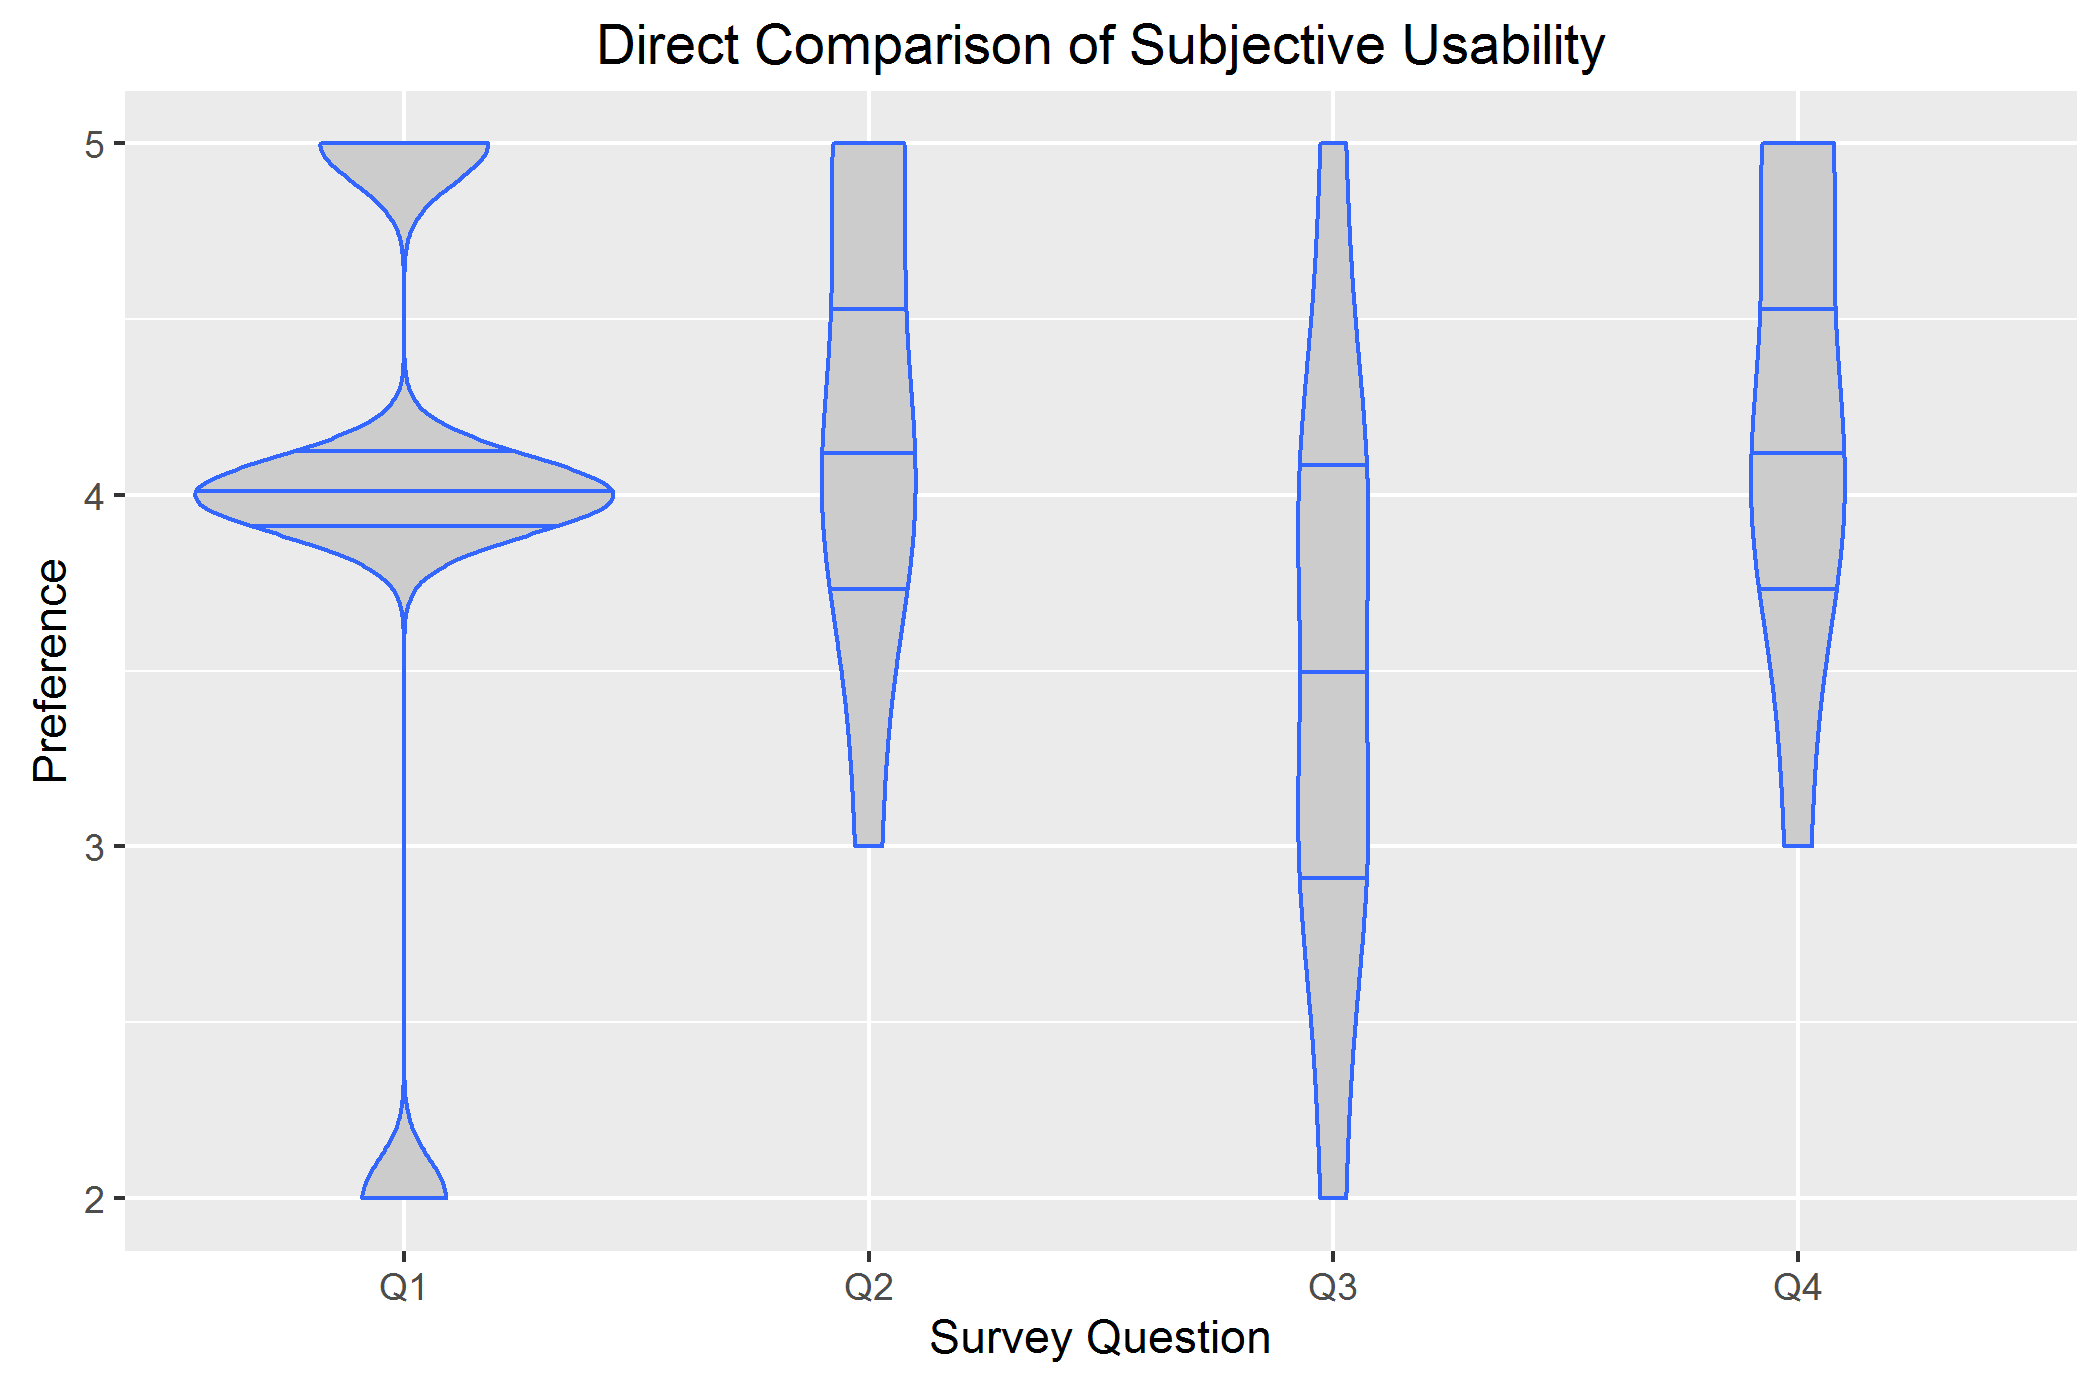
\includegraphics[width=.8\linewidth]{direct_comparison_violin}
  \caption{A violin plot indicating the distribution of responses. The plot is wider at sections where there were more responses with that value.}
  \label{fig:subjective_direct}
\end{figure}

%
\subsection{Task Performance and Task Effort}
\begin{table*}
    \centering
    \begin{tabular}{| c | c | c | c | c | c | c | c |}
    \hline
    \multicolumn{8}{|c|}{Average Task Completion Times (s) by Task} \\
    Interface Version & T1 & T2 & T3 & T4 & T5 & T6 & T7 \\
    \hline
    \hline
    Current           & 104.0 &  93.7 &  44.3 &  95.5 & 107.9 &  37.1 &   16.1 \\
    \hline
    In-Development    & 144.4 &  79.8 &  48.2 &  93.2 &  76.9 &  45.9 &   11.9 \\
    \hline
    \hline
    Difference        & 40.4  & -13.9 &   3.9 &  -2.3 & -31.0 &   8.8 &    4.2 \\
    \hline
    \% Difference     & 38.8  & -14.8 &   8.8 &  -2.4 & -28.7 &  23.7 &   26.1 \\
    \hline
    \hline
    Significant (Y?) &        &       &       &       &       &       &       \\
    \hline
    p-Value          & 0.543  & 0.470 & 0.729 & 0.928 & 0.408 & 0.457 & 0.264 \\
    \hline
    F-Value          & 0.389  & 0.552 & 0.125 & 0.009 & 0.729 & 0.586 & 1.355 \\
    \hline
    \end{tabular}
    
    \caption{Average task completion times by interface version. Difference and percent difference is computed relative to the \emph{current} version values.}
    \label{tab:avg_task_time}
\end{table*}

The average task completion time (\emph{Task Performance}) ranged from 11.9 seconds at the fastest, to 144.4 seconds at the slowest. The fastest and slowest times both occurred for participants while using the \emph{in-development} version of the interface. Averaging across tasks, the \emph{in-development} version was roughly 2\% slower. However, the results were not statistically significant ($F_{1,8} = 1.355$, $p > 0.264$, at best); to remark on the effect of \emph{Interface Version} on \emph{Task Performance} other than to say that there may not be one, is not possible. This is not entirely bad news - to say that there might be no effect is to say that the \emph{in-development} version is not less navigable than the \emph{current} one. 

\begin{figure}[h!]
  \centering
  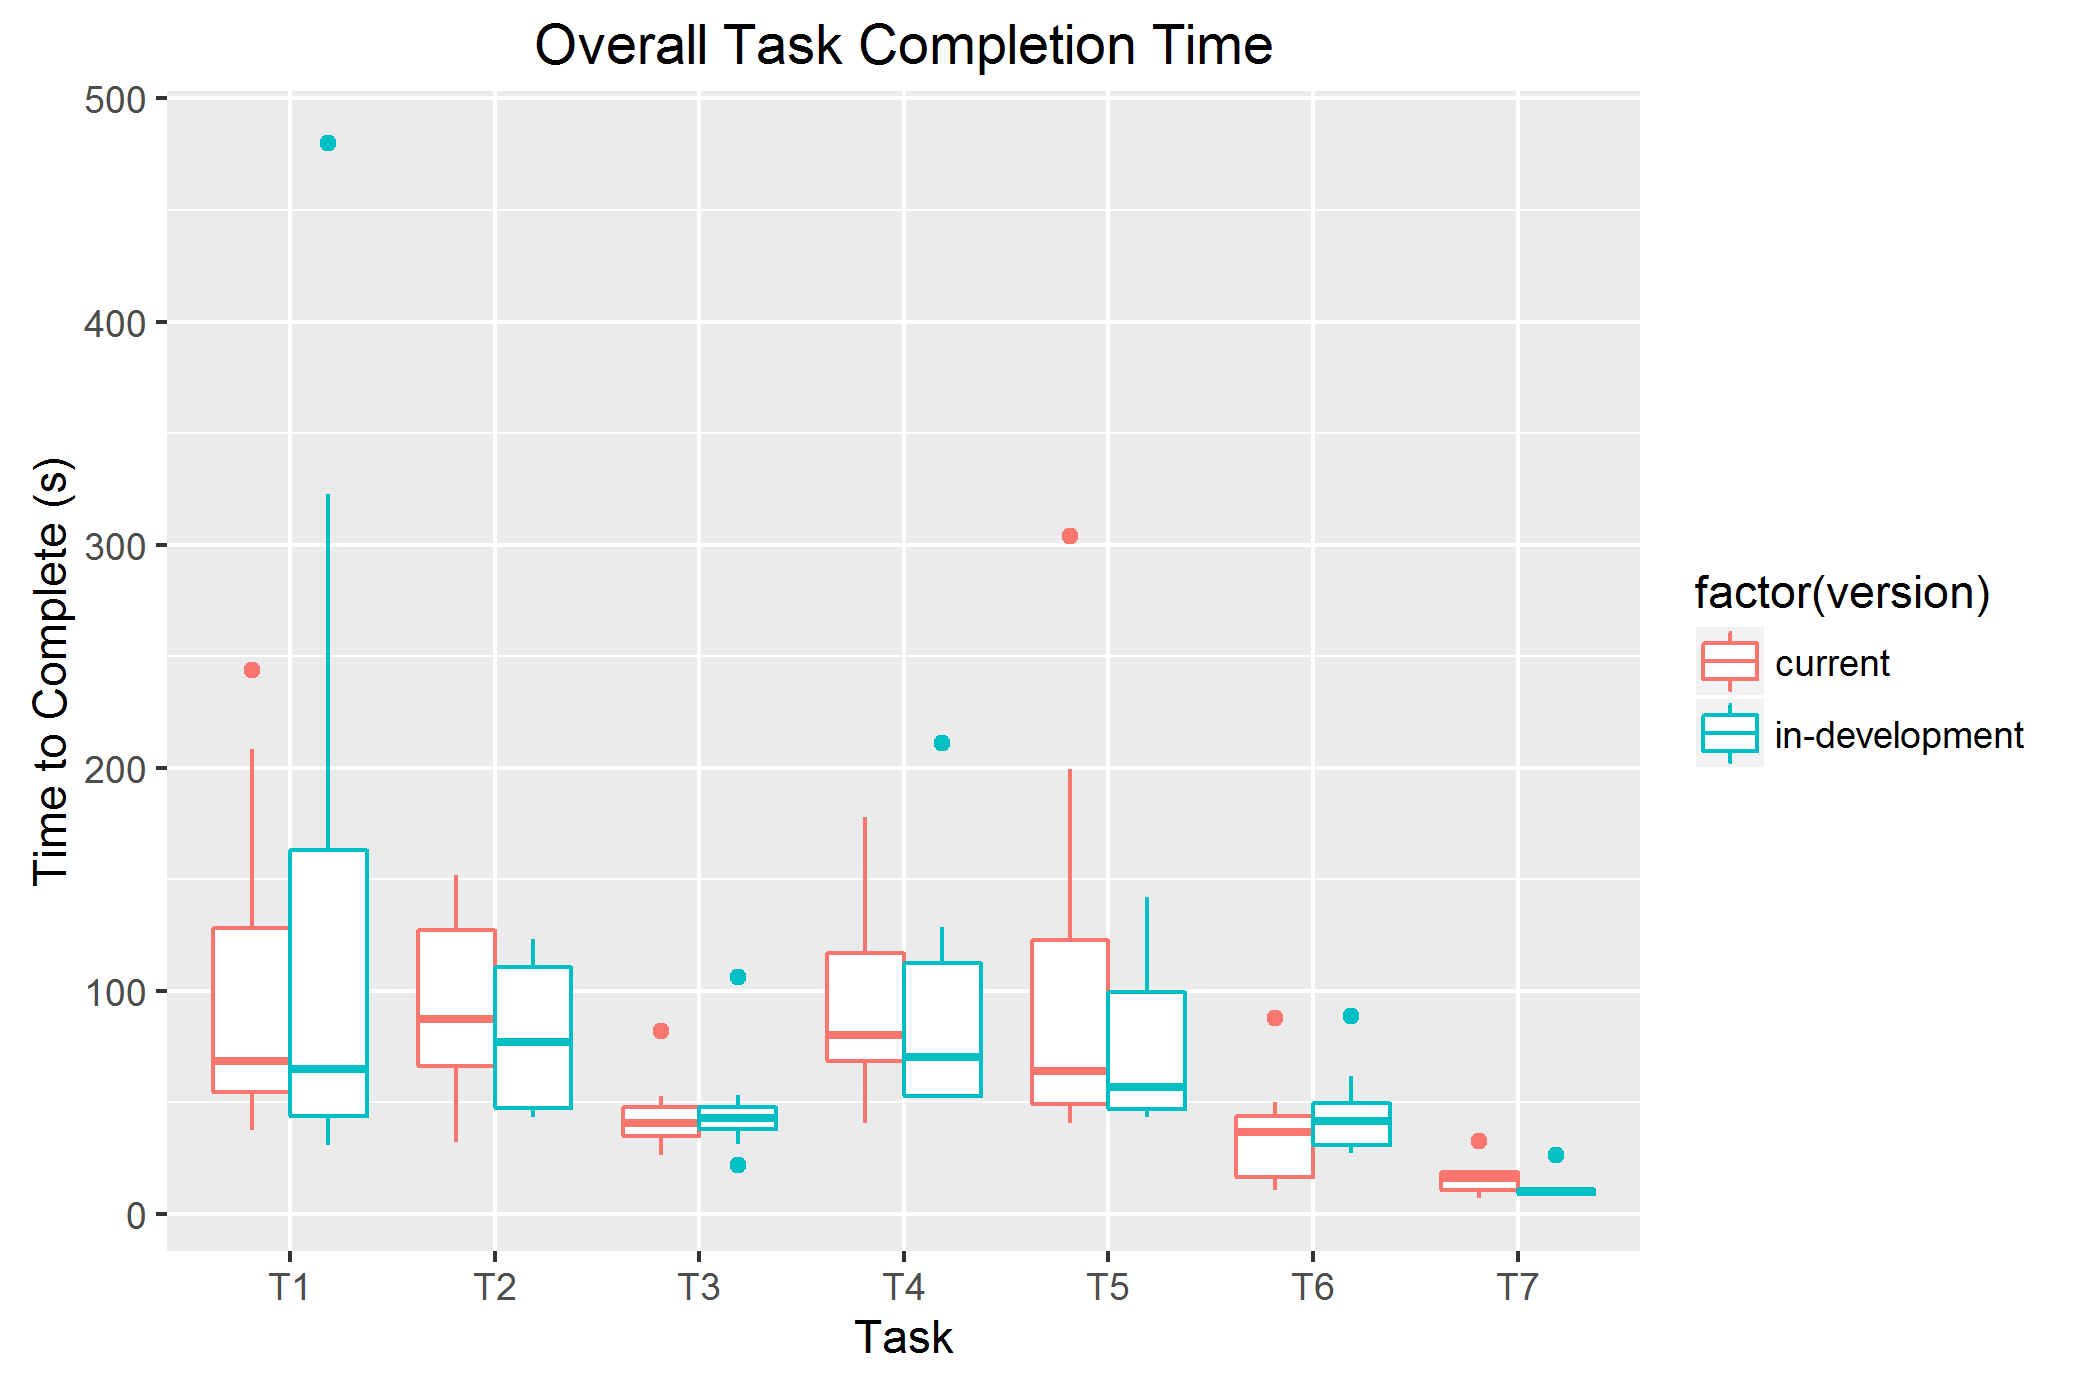
\includegraphics[width=.8\linewidth]{overall_task_completion}
  \caption{A box and whisker plot indicating the nature of the task completion times for the tasks participants were given. Dots represent outliers.}
  \label{fig:boxplot_task_time}
\end{figure}

%
\subsection{Task Effort}
\begin{figure}[h!]
  \centering
  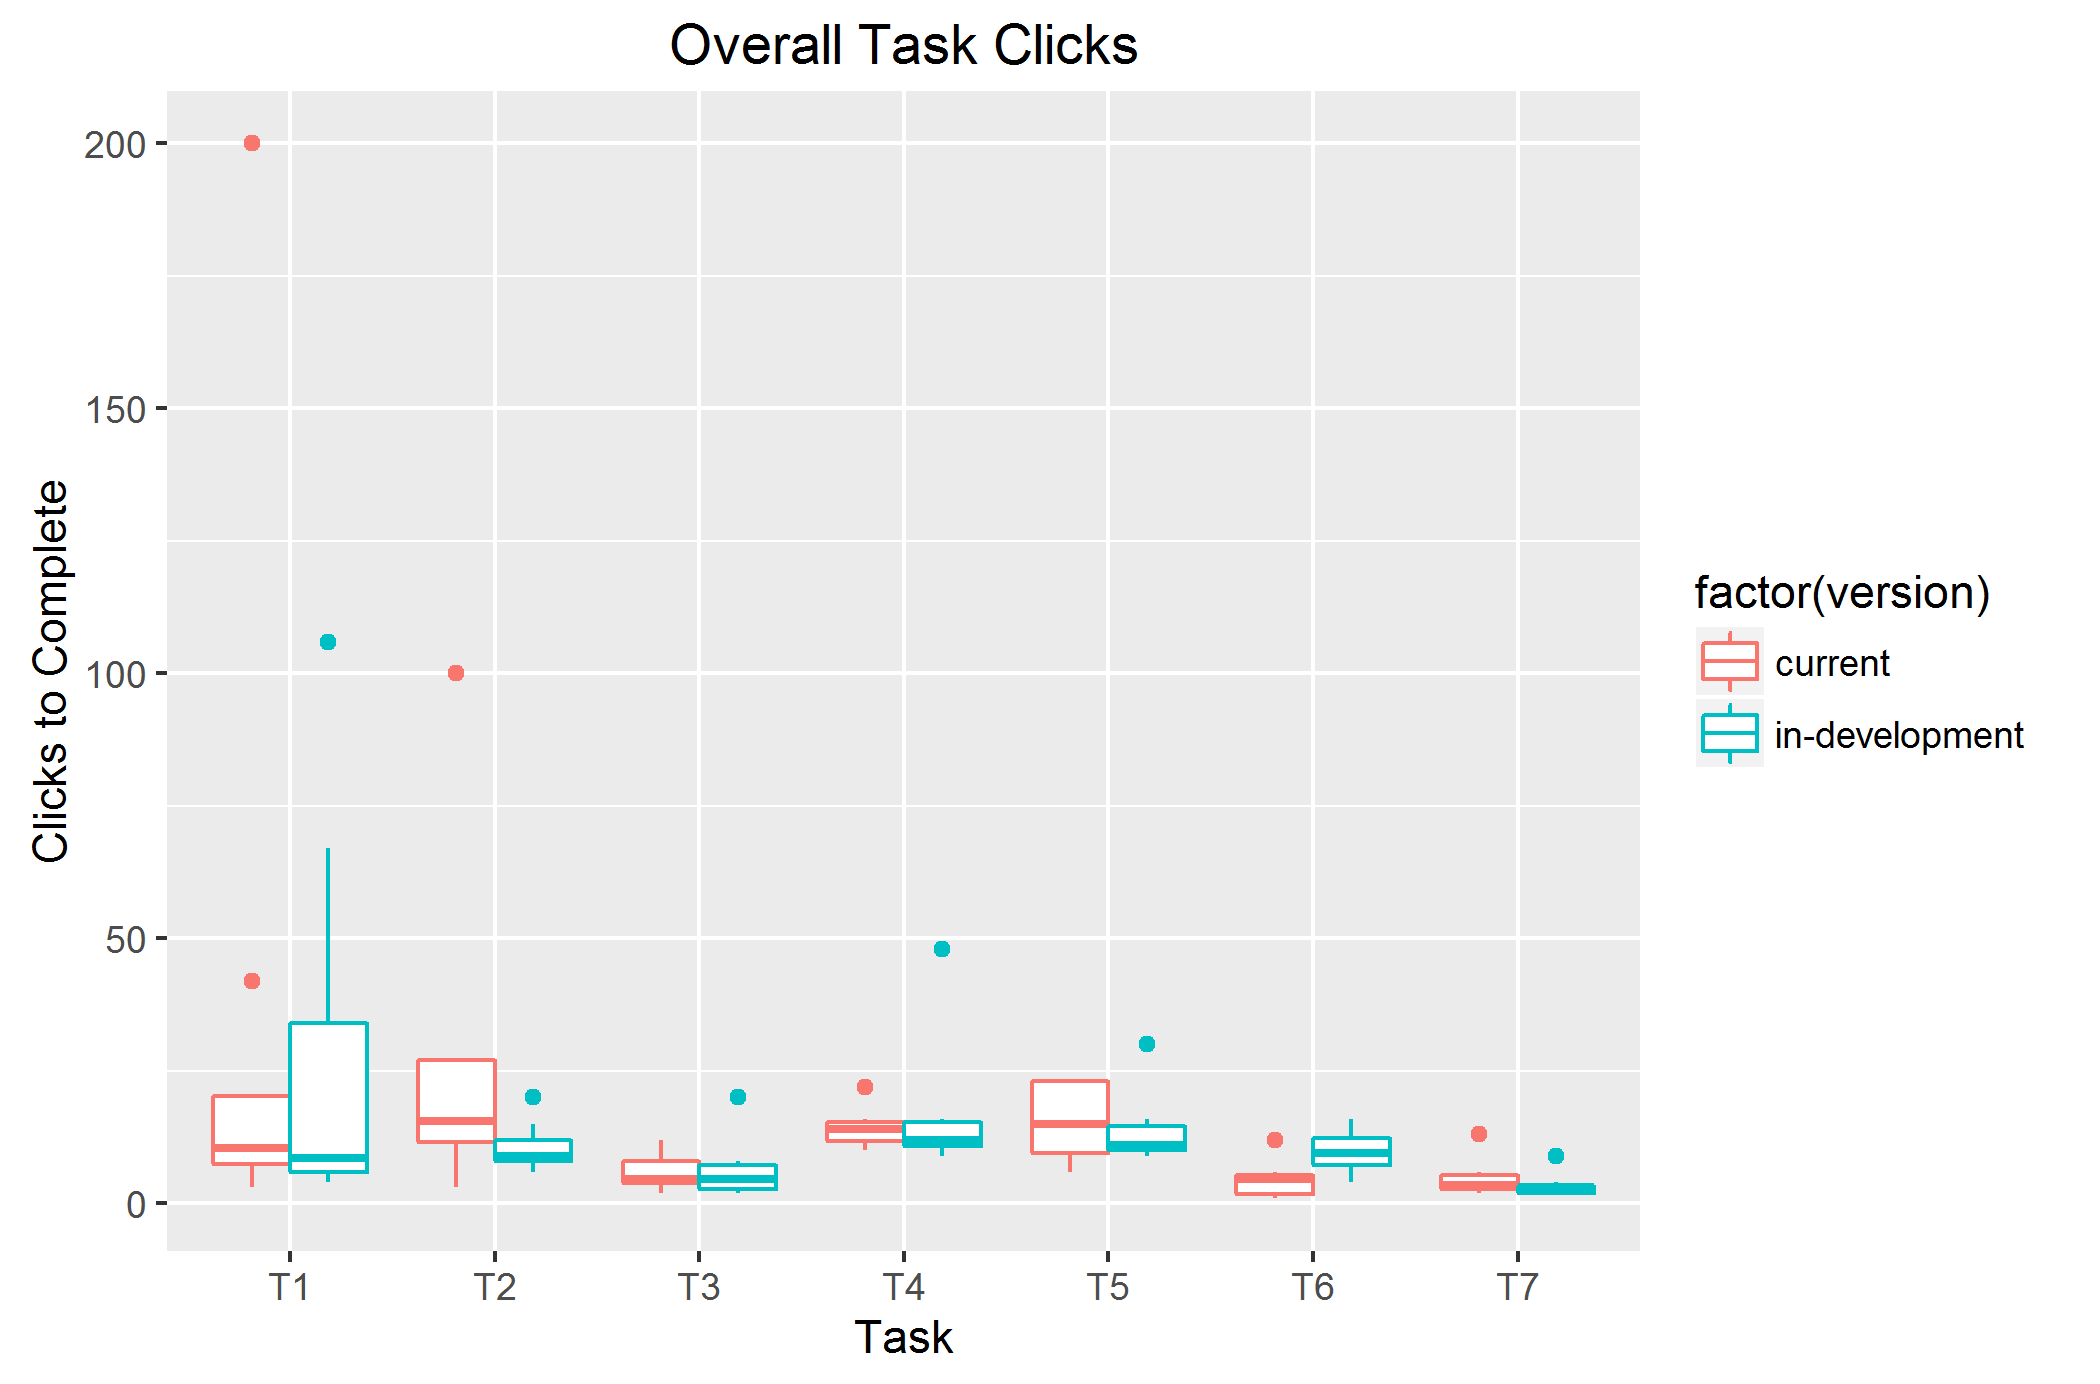
\includegraphics[width=.8\linewidth]{overall_task_clicks}
  \caption{A box and whisker plot indicating the number of clicks required to complete the tasks participants were given. Dots represent outliers.}
  \label{fig:boxplot_avg_clicks}
\end{figure}

The average number of clicks required (\emph{Task Effort}) ranged across tasks from 3.5 to 36.6. Averaging over all tasks, the \emph{in-development} version required 18.8\% fewer clicks than the \emph{current} version to complete tasks. Similar to \emph{Task Performance}, though, statistical significance was not achieved ($F_{1,8} = 1.885$, $p > 0.191$, at best), with one exception ($F_{1,8} = 7.215$, $p < 0.05$). Again, it would not be possible to remark on the effect of \emph{Interface Version} on \emph{Task Effort}. As with \emph{Task Performance}, this is not necessarily bad news because it indicates that the \emph{in-development} version has not made things worse.

For the one statistically significant task that we can remark on, however, it is an interesting case because the \emph{in-development} version actually performed worse, requiring roughly twice as many clicks. This particular task was a photo finding task in the image gallery. The two interfaces differed slightly in photo arrangement in the gallery, but also in that the \emph{in-development} version allows users to scroll between enlarged versions of photos, like a slide show. This would, of course, stimulate more clicking among participants, although it is conceivable that this is actually desirable in an image gallery where users aren't always focused on finding specific images, but more likely to be simply browsing.

\begin{table*}
    \centering
    \begin{tabular}{| c | c | c | c | c | c | c | c |}
    \hline
    \multicolumn{8}{|c|}{Average Clicks to Complete a Task} \\
    Interface Version & T1 & T2 & T3 & T4 & T5 & T6 & T7 \\
    \hline
    \hline
    Current           & 36.6 & 26.0 &  6.0 & 14.3 & 15.4 &  4.5 &  4.8 \\
    \hline
    In-Development    & 28.6 & 10.8 &  6.4 & 16.6 & 13.9 &  9.6 &  3.5 \\
    \hline
    \hline
    Difference        & -10.0 & -15.2 & 0.4 & 2.3 & -1.5 &  5.1 &  -1.3 \\
    \hline
    \% Difference     & -27.3 & -58.5 & 6.7 & 16.1 & -9.7 & 113.3 & -27.1 \\
    \hline
    \hline
    Significant (Y?) &       &       &       &       &       &     Y &       \\
    \hline
    p-Value          & 0.773 & 0.191 & 0.882 & 0.625 & 0.678 & 0.018 & 0.425 \\
    \hline
    F-Value          & 0.086 & 1.885 & 0.023 & 0.250 & 0.180 & 7.215 & 0.676 \\
    \hline
    \end{tabular}
    
    \caption{Average task completion times by interface version. Differences and Percent Differences are computed relative to the \emph{current} version values.}
    \label{tab:avg_clicks}
\end{table*}

%
\subsection{Feedback and Observations}
Perhaps the richest results of the experiment were the ones that could not be measured. Feedback from participants and observations from researchers will provide valuable feedback on what specifically can be improved about the NRDC.

\subsubsection{Navigating Between Tasks}
Much of the experiment was focused on helping users to navigate effectively and pleasantly. It was not statistically significant that users could navigate between tasks any more quickly, but the feedback on the quality of the site was more positive for the \emph{in-development} version.

Many of the participants requested that there be some kind of omni-present "nav bar" to help them navigate effectively, as there were complaints about getting lost, or being unable to return to a previous screen easily. The \emph{in-development} version sought to address this by, instead of creating a new tab, presenting the service being accessed in the same window. However, the lack of said "nav bar" or an explicit widget to close the sub-window did result in minor confusion for some participants.

\subsubsection{Geo-spatial Data Search}
In general, participants suffered the largest difficulties using the Geo-spatial Data Search. There was a large number of controls and pieces of information for participants to understand, and this led to frustration for participants.

One of the most requested features was actually a list or some kind of search functionality to help users select the target location in the Geo-spatial Data Search. There is a list feature for just this purpose, but few (2) of the users noticed it, indicating that it should be made more prominent.

Of interest is the fact that there is a video-tutorial available on the Geo-spatial Data Search page. However, none of the participants used it. We did have a test participant (excluded in the data, used to test our procedure) who did use the tutorial, the sole instance of tutorial use. The general reasoning among participants (and the researchers) was that the task should be simple, and watching a video would be an annoying waste of time.

\subsubsection{Current Conditions vs. Geo-spatial Data Search}
In all task sets, the first task required the participant to use the Current Conditions service. We observed that almost all of the participants used the Geo-spatial Data Search initially instead, thinking that the Geo-spatial Data Search would provide current data along with any other data.

Likely contributing this misconception was the relative positioning of the links for the Geo-spatial Data Search and the Current Conditions services. Both are located in a drop-down menu simply labeled "Data", but Current Conditions is listed further down the list. We observed participants mousing over "Current Conditions" several times and using the Geo-spatial Data Search instead.

We make the recommendation that items should be re-ordered, or perhaps decorated to emphasize the information they can provide to a user.

\begin{table*}
    \centering
    \begin{tabular}{| c | p{15cm} |}
    \hline
    \multicolumn{2}{|c|}{Common Criticisms and Observations About the NRDC} \\
    Source & Criticism/Observation \\
    \hline
    \hline
    Participant & (Referring to the current NRDC interface) "Navigation between some of the services is difficult as the nav bar disappears." \\
    \hline
    Participant & (Referring to the in-development NRDC interface and the way it presents services in the same window) "Exiting a pop up window for services may not be intuitive for some people." \\
    \hline
    Participant & "On the [geo-spatial] search, it was confusing at first as to which parts of the interface to click first, and what conditions would be needed to be met to download / visualize data." \\
    \hline
    Participant & "Keep a persistent nav bar  at top so it's always possible to get back and easy to navigate." \\
    \hline
    Participant & "I feel as though the image retrieval (the one which makes composite videos) UI throws too much information at you all at once." \\
    \hline
    Researcher  & The list drop-down for selecting locations in the geo-spatial data search should be made more prominent. \\
    \hline
    Researcher  & The links to the services in the NRDC home page should be re-ordered by relevance and be made more distinguishable from one another. \\
    \hline
    Researcher  & If the Webcam Streams are deprecated, they should be clearly marked as such or removed. \\
    \hline
    \end{tabular}
    
    \caption{A sampling of the criticisms and observations the experiment produced.}
    \label{tab:criticisms_observations}
\end{table*}

%
%
\section{Conclusion}
%
\subsection{Summary}
Two versions of interfaces for the NRDC were compared, the \emph{current} and \emph{in-development} versions. While it is unclear if either version is superior to the other in terms of user performance, the \emph{in-development} version is preferable to users in terms of aesthetics. On average, it was at least preferable to the \emph{current} interface. Further, many points of improvement were determined through open-ended user feedback and researchers' observations. These points most directly indicated improvements to the navigation of the NRDC and improved visibility of key features and controls.

%
\subsection{Future Work}
As mentioned, the feedback and performance ratings from the participants yielded an abundance of clarity in regards of future developments. The data services, especially the Geo-spatial Data Search, clearly lack in a uniform interface, causing users a deal of confusion. In future iterations, this will be addressed alongside a more intuitive placement of elements for the Geo-spatial Data Search interface. Elements of all data service interfaces will be more pronounced and many existing elements will be minimized in order to avoid bombarding a user with an overabundance of actions. Overall, each data service will reflect a more intuitive approach whilst retain the same functionality it always had.

In addition, the interface of the website itself will undergo navigational changes, especially in regards to the Geo-spatial Data Search and the Current Events. The massive amount of confusion in which participant had dealing with the Current Events service indicates a strong need for revisions. In future iterations, the navigation will strongly emphasize the difference between data services. As to the question of having the data services appearing on the same page or in separate pages, revisions will be made initially to the same page design in the form of the exit button before possibly resorting to separate pages. Current research offers insight on how to best implement such a nav bar\cite{horizontal_nav_bar}, another method navigability could be improved.
%
\subsection{Acknowledgements}
This material is based in part upon work supported by the National Science Foundation under grant number IIA-1301726. Any opinions, findings, and conclusions or recommendations expressed in this material are those of the authors and do not necessarily reflect the views of the National Science Foundation. 

\bibliographystyle{abbrv}
\bibliography{Paper_Team_02}

%\balancecolumns 

\end{document}
